\phantomsection
\chapter*{প্রথম অধ্যায়ের নাম}
\addcontentsline{toc}{chapter}{প্রথম অধ্যায় (সূচীপত্রে)}
\markright{হেডার প্রথম}

\section*{(১)}
\addcontentsline{toc}{section}{(১) (সূচীপত্রে)}

\BanglaDummyText
\BanglaDummyText

\section*{(২)}
\addcontentsline{toc}{section}{(২) (সূচীপত্রে)}

\BanglaDummyText
\begin{figure}
	\centering
	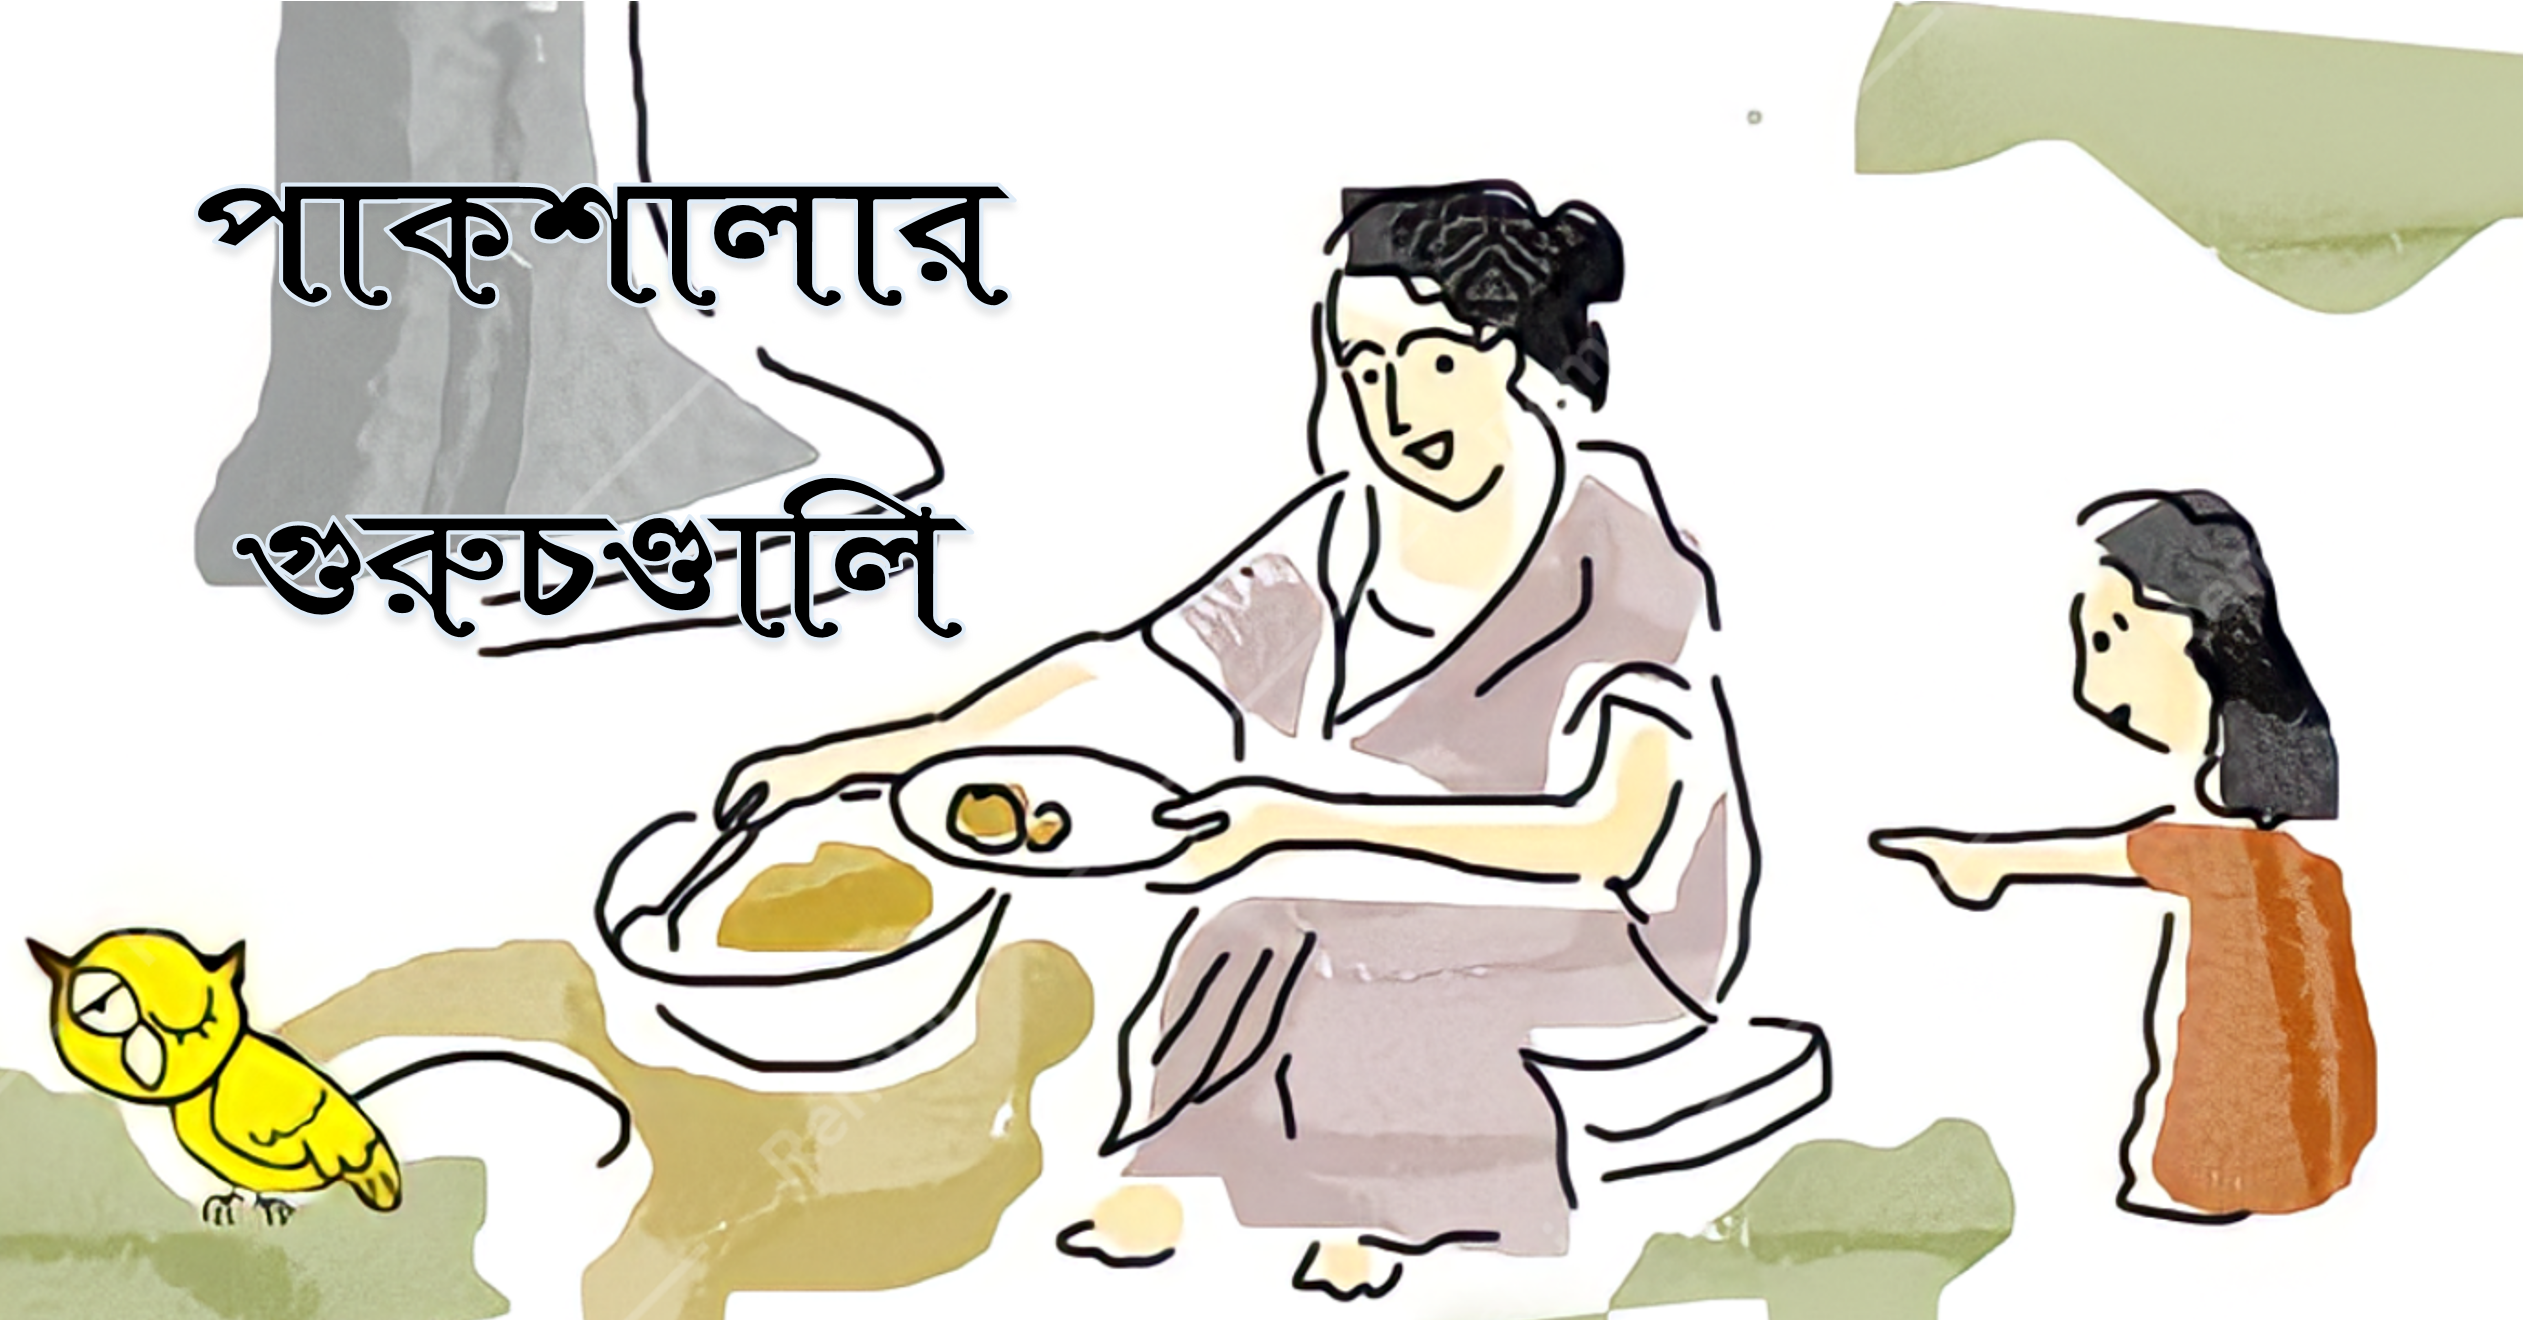
\includegraphics[width=\linewidth]{Images/DemoPic1.png}
	\caption{\small \textbf{ডেমো ক্যাপশন}}
\end{figure}

\BanglaDummyText
\begin{quotation}
	\textit{\BanglaDummyText}
\end{quotation}
\BanglaDummyText

\vskip 30pt
\scriptsize
	\textbf{সূত্র:}
	\begin{enumerate}%[label={}]
		\item ১২০৫-১২০৬ খ্রিস্টাব্দের দিকে ইখতিয়ার উদ্দিন মুহম্মদ বখতিয়ার খলজী নামের একজন তুর্কী বংশোদ্ভূত সেনাপতি রাজা লক্ষ্মণ সেনকে পরাজিত করে সেন রাজবংশের পতন ঘটান।
		\item ১৭৫৭ খ্রিস্টাব্দে ব্রিটিশ ইস্ট ইন্ডিয়া কোম্পানি পলাশীর যুদ্ধে জয়লাভের মাধ্যমে বাংলার শাসনক্ষমতা দখল করে
		\item ১৮৫৭ খ্রিস্টাব্দের সিপাহী বিপ্লবের পর কোম্পানির হাত থেকে বাংলার শাসনভার ব্রিটিশ সাম্রাজ্যের সরাসরি নিয়ন্ত্রণে আসে
		\item ভারতীয় উপমহাদেশের দেশভাগের সময় ১৯৪৭ খ্রিস্টাব্দে ধর্ম গরিষ্ঠতার ভিত্তিতে পুনর্বার বাংলা প্রদেশটিকে ভাগ করা হয়। পাকিস্তান এর প্রদেশ হিসাবে জন্ম নেয় পূর্ব পাকিস্তান 
		\item ১৯৭১ সালে ৯ মাস ব্যাপী রক্তক্ষয়ী যুদ্ধের মাধ্যমে পাকিস্তানী হানাদার বাহিনীকে পরাজিত করে স্বাধীনতা লাভ করে বাংলাদেশ 
	\end{enumerate}
